% !TEX root = ../lab3.tex
\section{Техническое задание}

\begin{itemize}
	\item Подобрать черно-белое изображение;
	\item Провести для него сглаживание по Гауссу;
	\item Определить границы сглаженного изображения с помощью Лапласиана;
	\item Добиться повышения резкости границ исходного изображения, используя найденные границы из предыдущего шага.
\end{itemize}

\section{Ход работы}

Для выполнения работы был разработан класс EdgeStrength с использованием библиотек OpenCV и Matplotlib на языке Python (листинг \vref{lst:edgestrength}). Пример его использования приведен в листинге \cref{lst:mainpy}, а использованные зависимости для virtualenv --- в листинге \cref{lst:requirements}.

Исходное изображение представлено на \vref{pic:grey}.

\begin{figure}[H]
	\centering
	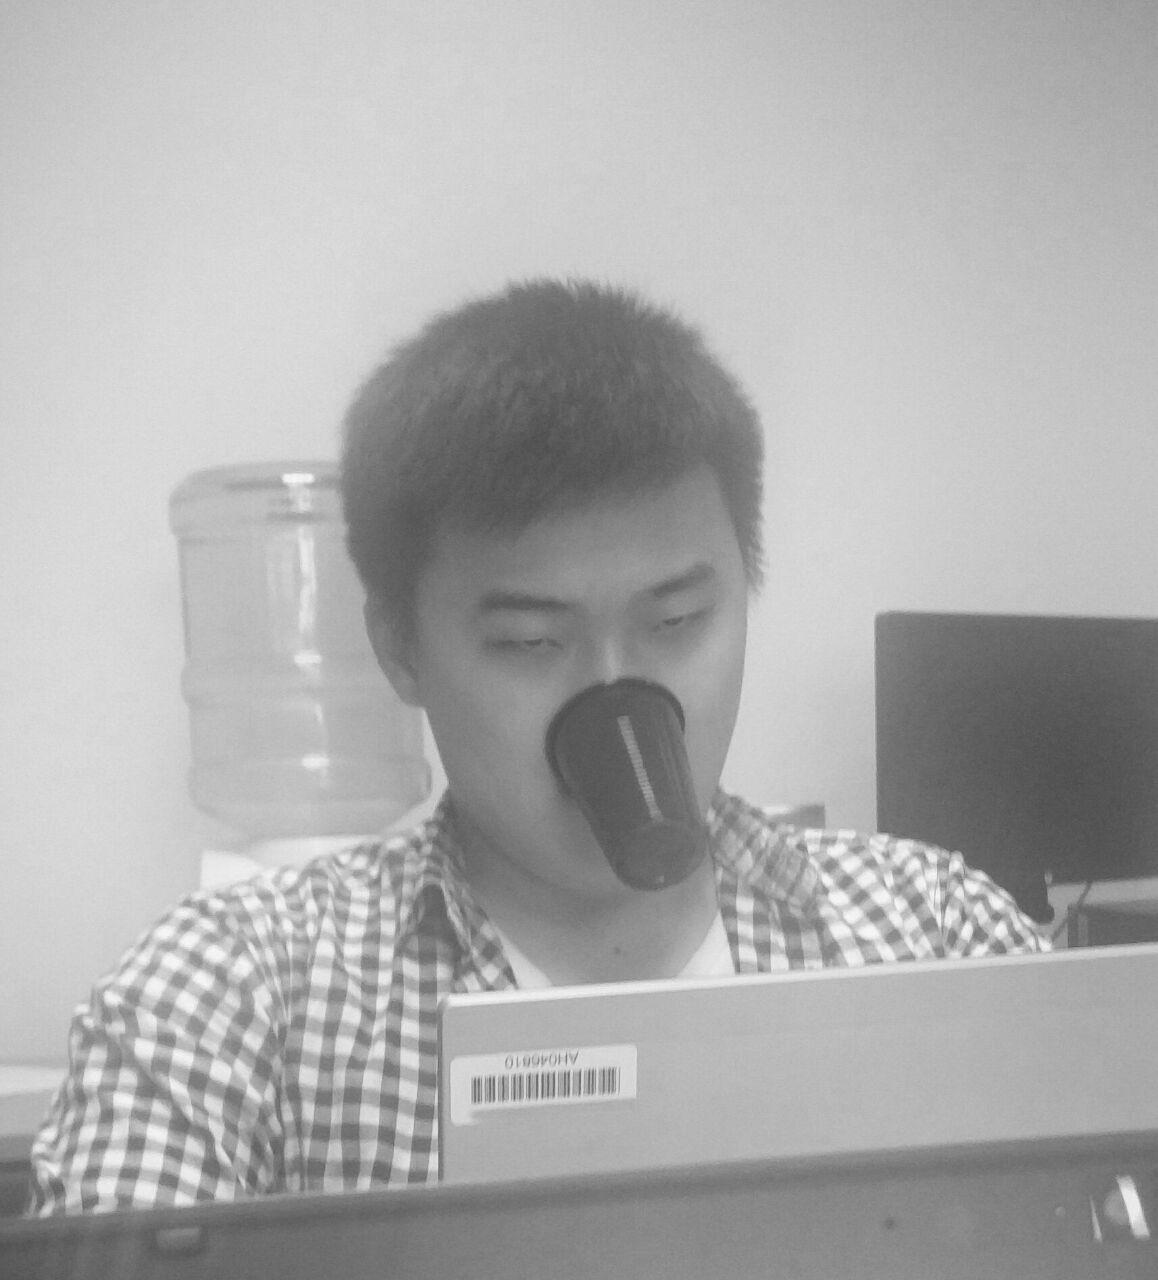
\includegraphics[width=\textwidth]{grey}
	\caption{Черно-белое изображение}
	\label{pic:grey}
\end{figure}

\subsection{Сглаживание по Гауссу}

Проведем сглаживание исходного изображения по Гауссу (\vref{pic:gauss3}), применив ядро свёртки 
$\begin{bmatrix}
    1 & 2 & 1 \\
    2 & 4 & 2 \\
    1 & 2 & 1
\end{bmatrix}$. Для этого воспользуемся методом \texttt{gaussSmoothing} класса EdgeStrength.

\begin{figure}[H]
	\centering
	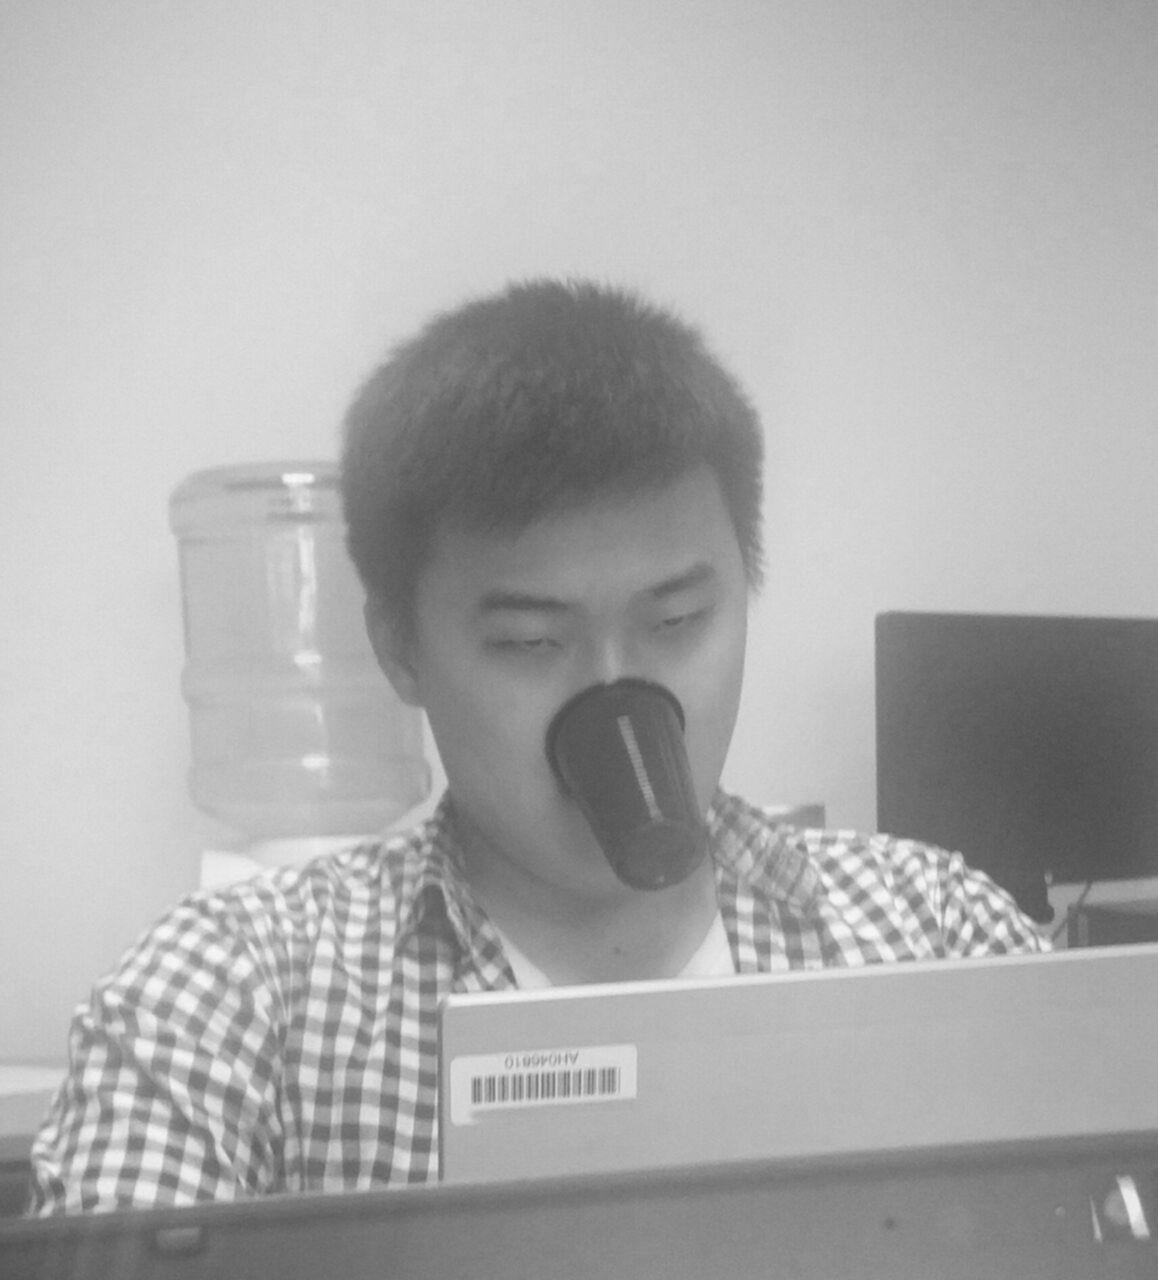
\includegraphics[width=\textwidth]{3_gauss3}
	\caption{Cглаживание по Гауссу}
	\label{pic:gauss3}
\end{figure}

\subsection{Определение границ}

Проведем определение границ с помощью Лапласиана (\vref{pic:lap3}), применив ядро свёртки 
$\begin{bmatrix}
    -1 & -1 & -1 \\
    -1 &  8 & -1 \\
    -1 & -1 & -1
\end{bmatrix}$. Для этого воспользуемся методами \texttt{\_laplacian} и \texttt{\_lsLaplacian} (для линейного сжатия лапласиана) класса EdgeStrength.

\begin{figure}[H]
	\centering
	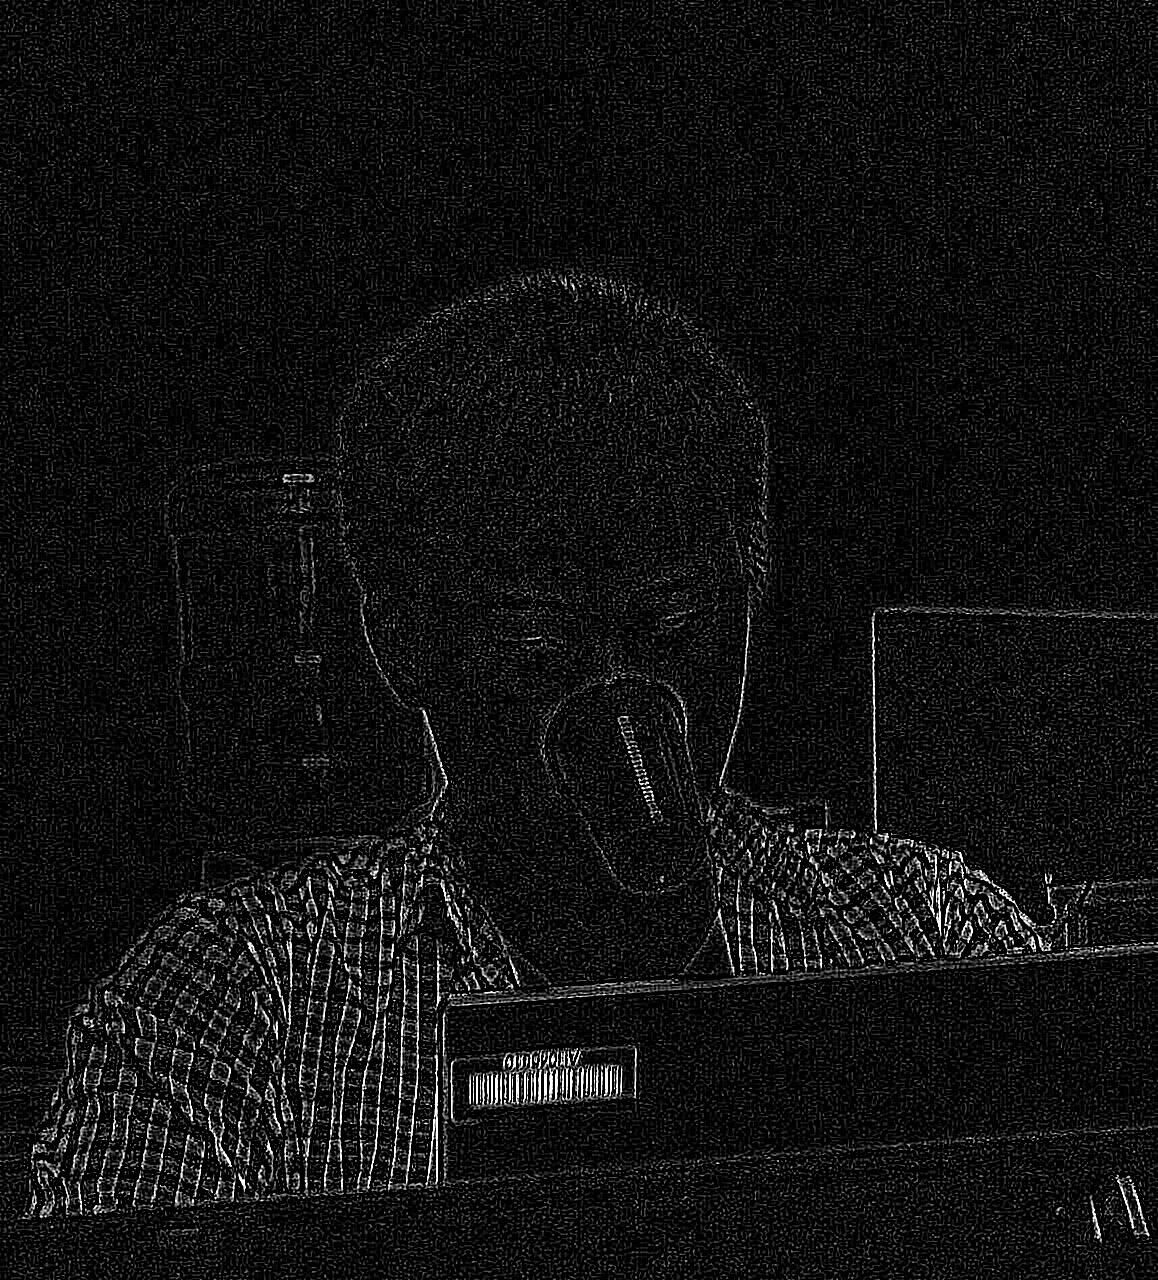
\includegraphics[width=\textwidth]{4_lap3}
	\caption{Определение границ Лапласианом}
	\label{pic:lap3}
\end{figure}

\subsection{Повышение резкости границ изображения}

Проведем повышение резкости границ изображения (\vref{pic:res3}) путем умножения пикселей исходного изображения на определенные Лапласианом границы. Для этого воспользуемся методом \texttt{strengtheningEdges} класса EdgeStrength.

\begin{figure}[H]
	\centering
	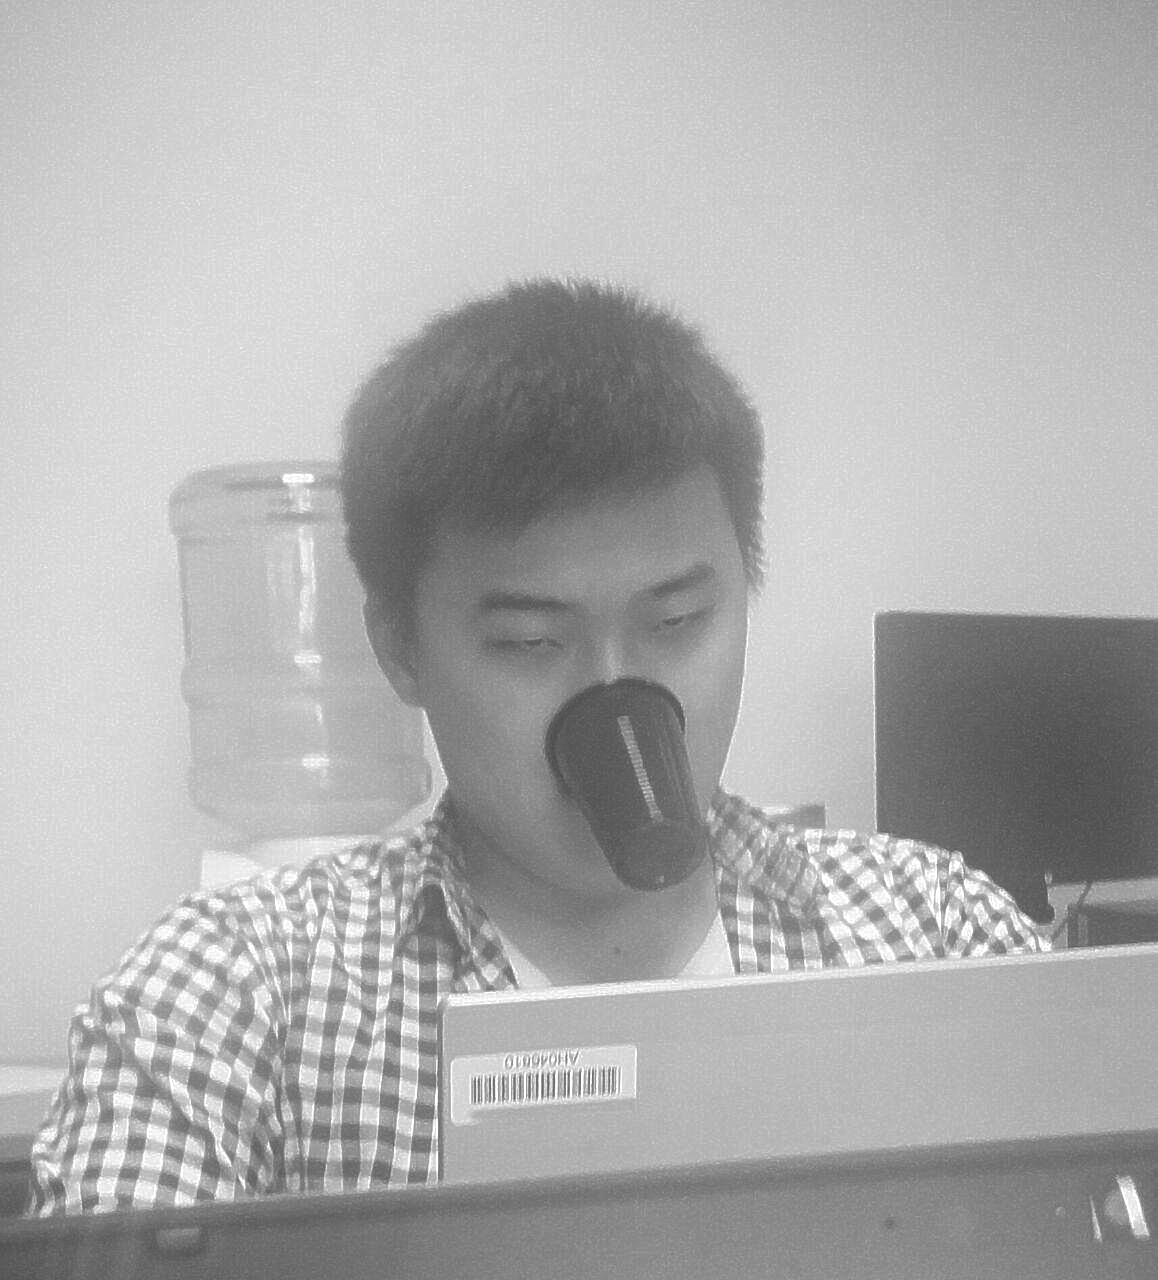
\includegraphics[width=\textwidth]{5_res3}
	\caption{Повышение резкости границ изображения}
	\label{pic:res3}
\end{figure}

\section{Выводы}

В данной работе было проведено сглаживание по Гауссу, определение границ с помощью Лапласиана, а затем совмещение полученного изображения с исходным для повышения резкости границ изображения.

В результате проделанных действий получилось изображение с более четкими границами, но вследствие этого границы стали выглядеть зашумленными.
